\documentclass[a4paper, titlepage,12pt]{article}
\usepackage[margin=3.7cm]{geometry}
\usepackage[utf8]{inputenc}
\usepackage[T1]{fontenc}
\usepackage[swedish,english]{babel}
\usepackage{csquotes}
\usepackage[hyphens]{url}
\usepackage{amsmath,amssymb,amsthm, amsfonts}
\usepackage[yyyymmdd]{datetime}
\usepackage{graphicx}
\usepackage{longtable}
\usepackage{float}

\title{Assignment 1 \& 2, TCP/IP Internetworking}
\author{Adam Temmel (adte1700), Fredrik Sellgren (frse1700),\\Oscar Fredriksson (osfr1701)}

\begin{document}
	\maketitle
	\section{Preparation: Subnetting}\label{sec:introduction}

	First, we had to determine our IP-range.\\

	\begin{figure}[h!]
		\begin{center}
			Fredrik's birthday:\\
			$(89\cdot02+08) \ mod \ 223 = 186$\\
			Oscar's birthday:\\
			$(9\cdot02+04) \ mod \ 255 = 200$\\
			Adam's birthday:\\
			$(9\cdot11+16) \ mod \ 255 = 85$\\
			\caption{All preliminary IP arithmetic}
		\end{center}
	\end{figure}

	This gave us the resulting IP-range of $186.200.85/20$.

	\subsection{What is the network-ID of your groups subnet?}

		\begin{center}
			$186.200.85.0 \ bitwise \ and \ 255.255.240.0 = 186.200.80.0$\\
		\end{center}

	\subsection{What is the broadcast address of your groups subnet?}

		\begin{center}
			$186.200.85.0 \ bitwise \ or \ 0.0.15.255 = 186.200.95.255$\\
		\end{center}

	\subsection{How many hosts in total can this subnet hold?}

		\begin{center}
			$2^{32-20} - 2 = 2^{12} - 2 = 4096 - 2 = 4094$\\
		\end{center}

	\section{Further network planning}

		The network requirements for this assignment are presented in \textit{figure~\ref{netreq}}.

		\begin{figure}[h!]
			\begin{center}
				\begin{tabular}{|c|c|}
					\hline
					\textbf{Device} & \textbf{Number of hosts} \\
					\hline
					RT-A & 2100 \\
					\hline
					RT-B & 1000 \\
					\hline
					RT-C & 300 \\
					\hline
					RT-D & 600 \\
					\hline
					Link nets & 4 \\
					\hline
				\end{tabular}
				\caption{Network requirements}
				\label{netreq}
			\end{center}
		\end{figure}

		It then follows that our original subnet needs to be subnetted further in order to provide these specific requirements.
		Our proposed new subnets are shown in \textit{figure~\ref{suggestedconfig}}.

		\begin{figure}[h!]
		\begin{center}
			\begin{tabular}{|c|c|}
				\hline
				RT-A & 2100 hosts \\
				\hline
				186.200.80.0/21 & 2046 hosts \\
				\hline
				186.200.95.0/26 & 62 hosts \\
				\hline
			\end{tabular}
		\end{center}

		\begin{center}
			\begin{tabular}{|c|c|}
				\hline
				RT-B & 1000 hosts \\
				\hline
				186.200.88.0 & 1022 hosts \\
				\hline
			\end{tabular}
		\end{center}

		\begin{center}
			\begin{tabular}{|c|c|}
				\hline
				RT-C & 300 hosts \\
				\hline
				186.200.94.0/24 & 254 hosts \\
				\hline
				186.200.95.64/26 & 62 hosts \\
				\hline
			\end{tabular}
		\end{center}

		\begin{center}
			\begin{tabular}{|c|c|}
				\hline
				RT-D & 600 hosts \\
				\hline
				186.200.92.0/23 & 510 hosts \\
				\hline
				186.200.95.128/26 & 62 hosts \\
				\hline
				186.200.95.192/27 & 30 hosts \\
				\hline
			\end{tabular}
		\end{center}

		\begin{center}
			\begin{tabular}{|c|c|}
				\hline
				\textbf{Connection} & \textbf{Designated Address} \\
				\hline
				RT-A → RT-B & 186.200.95.224/30\\
				\hline
				RT-A → RT-C & 186.200.95.228/30\\
				\hline
				RT-D → RT-B & 186.200.95.232/30\\
				\hline
				RT-D → RT-C & 186.200.95.236/30\\
				\hline
			\end{tabular}
		\end{center}
		\caption{All routers and their respective subnets}
		\label{suggestedconfig}
	\end{figure}

	\section{Building the network}
		\subsection{Which group member was doing the configuration for this part?}

		\begin{figure}[h!]
			\begin{center}
				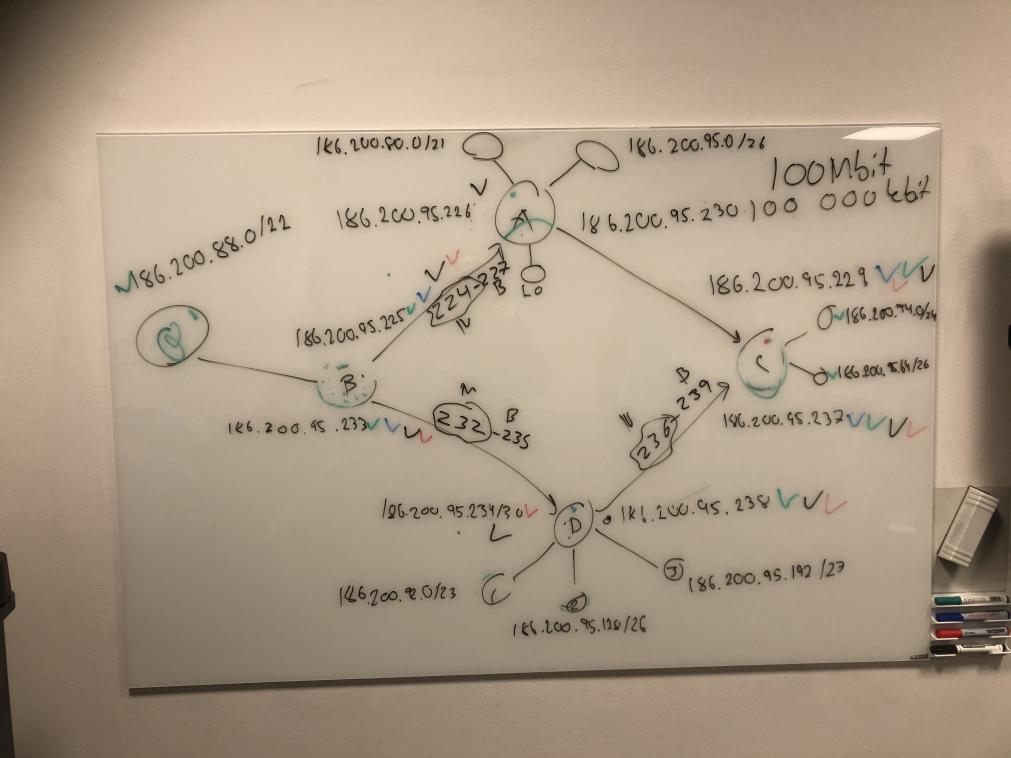
\includegraphics[scale=0.20]{./static_img.jpg}
			\end{center}
			\caption{A visual representation of the suggested configuration}
		\end{figure}

			We found it easiest to let one member connect to the system and mirror his screen on a large display. The idea here is that one group member could setup the network under the supervision of all other members. If all members could verify the validity of each command, the risk of misconfiguring the network should be minimized (This did not work out perfect in reality, as we did mess up at times). For this part, Fredrik Sellgren was responsible for typing in the requested commands.

		\subsection{Static routing}

		\subsubsection{List the static routes configured:}

			\begin{center}
		\begin{longtable}{|l|l|l|}

			\hline
			\textbf{Route} & \textbf{Hop} & \textbf{Explanation} \\
			\hline
			A → 186.200.94.0 & 186.200.95.229 & A →  C’s subnet with 254 hosts \\
			\hline
			A → 186.200.95.64 & 186.200.95.229 & A →  C’s subnet with 62 hosts \\
			\hline
			A → 186.200.95.238 & 186.220.95.229 & A →  D via C  \\
			\hline
			A → 186.200.95.234 & 186.200.95.225 & A →  D via B  \\
			\hline
			A → 186.200.88.0 & 186.200.95.225 & A →  B’s subnet with 1022 hosts \\
			\hline
			A → 186.200.92.0 & 186.200.95.238 & A →  D’s subnet with 510 hosts via C \\
			\hline
			A → 186.200.95.128 & 186.200.95.238 & A →  D’s subnet with 62 hosts via C \\
			\hline
			A → 186.200.95.192 & 186.200.95.238 & A →  D’s subnet with 30 hosts via C \\
			\hline
			A → 186.200.92.0 & 186.200.95.234 & A →  D’s subnet with 510 hosts via B \\
			\hline
			A → 186.200.95.128 & 186.200.95.234 & A →  D’s subnet with 62 hosts via B \\
			\hline
			A→ 186.200.95.192 & 186.200.95.234 & A →  D’s subnet with 30 hosts via B  \\
			\hline
			B → 186.200.80.0 & 186.200.95.226 & B →  A’s subnet with 2046 hosts \\
			\hline
			B → 186.200.95.0 & 186.200.95.226 & B →  A’s subnet with 62 hosts \\
			\hline
			B → 186.200.92.0 & 186.200.95.234 & B →  D’s subnet with 510 hosts \\
			\hline
			B → 186.200.95.128 & 186.200.95.234 & B →  D’s subnet with 62 hosts \\
			\hline
			B → 186.200.95.192 & 186.200.95.234 & B →  D’s subnet with 30 hosts \\
			\hline
			B → 186.200.95.237 & 186.200.95.234 & B →  C via D \\
			\hline
			B → 186.200.95.229 & 186.200.95.226 & B →  C via A \\
			\hline
			B → 186.200.95.64 & 186.200.95.234 & B →  C’s subnet with 62 hosts via D \\
			\hline
			B → 186.200.94.0 & 186.200.95.234 & B →  C’s subnet with 254 hosts via D \	\\
			\hline
			B → 186.200.95.64 & 186.200.95.226 & B →  C’s subnet with 62 hosts via A \\
			\hline
			B → 186.200.94.0 & 186.200.95.226 & B →  C’s subnet with 254 hosts via A \\
			\hline
			C → 186.200.92.0 & 186.200.95.238 & C →  D’s subnet with 510 hosts \\
			\hline
			C → 186.200.95.128 & 186.200.95.238 & C →  D’s subnet with 62 hosts \\
			\hline
			C → 186.200.95.192 & 186.200.95.238 & C →  D’s subnet with 30 hosts \\
			\hline
			C → 186.200.80.0 & 186.200.95.230 & C →  A’s subnet with 2048 hosts \\
			\hline
			C → 186.200.95.0 & 186.200.95.230 & C →  A’s subnet with 62 hosts \\
			\hline
			C → 186.200.95.225 & 186.200.95.230 & C →  B via A \\
			\hline
			C → 186.200.95.233 & 186.200.95.238 & C →  B via D \\
			\hline
			C → 186.200.88.0 & 186.200.96.225 & C →  B’s subnet with 1022 hosts via A \\
			\hline
			C → 186.200.88.0 & 186.200.96.233 & C →  B’s subnet with 1022 hosts via D \\
			\hline
			D → 186.200.88.0 & 186.200.95.233 & D →  B’s subnet with 1022 hosts \\
			\hline
			D → 186.200.94.0 & 186.200.95.237 & D →  C’s subnet with 254 hosts \\
			\hline
			D → 186.200.95.64 & 186.200.95.237 & D →  C’s subnet with 62 hosts \\
			\hline
			D → 186.200.95.230 & 186.200.95.237 & D →  A via C \\
			\hline
			D → 186.200.95.226 & 186.200.95.233 & D →  A via B \\
			\hline
			D → 186.200.80.0 & 186.200.95.230 & D →  A’s subnet with 2046 hosts via C \\
			\hline
			D → 186.200..95.0 & 186.200.95.230 & D →  A’s subnet with 62 hosts via C \\
			\hline
			D → 186.200.80.0 & 186.200.95.226 & D →  A’s subnet with 2046 hosts via B \\
			\hline
			D → 186.200.95.0 & 186.200.95.226 & D →  A’s subnet with 62 hosts via B \\
			\hline
			B → 200.169.248.12 & 186.200.95.226 & B →  A’s loopback  \\
			\hline
			C → 200.169.248.12 & 186.200.95.230 & C →  A’s loopback \\
			\hline
			D → 200.169.248.12 & 186.200.95.230 & D →  A’s loopback via C \\
			\hline
			D → 200.169.248.12 & 186.200.95.226 & D →  A’s loopback via B \\
			\hline
		\end{longtable}
		\begin{figure}[H]
		\caption{List of all static routes configured}
		\end{figure}
	\end{center}

		After this configuration we were able to ping all the subnets from all the routers across the board.

		\subsubsection{When issuing a ping from RT-D to the loopback on RT-A, what path will the ICMP-packet take and why?}

		The traceroute command shows the RTT for both the paths, but by summarising the partial time of the paths taken, we can gather that the packet goes from RT-D → RT-B → RT-A, as the ping command shows a time that is closer to the second path than the first.

\begin{verbatim}

RT-D#ping 200.169.248.12
Type escape sequence to abort.
Sending 5, 100-byte ICMP Echos to 200.169.248.12, timeout is 2 seconds:
!!!!!
Success rate is 100 percent (5/5), round-trip min/avg/max = 40/41/44 ms

RT-D#traceroute ip 200.169.248.12
Type escape sequence to abort.
Tracing the route to 200.169.248.12
VRF info: (vrf in name/id, vrf out name/id)
  1 186.200.95.233 12 msec
    186.200.95.237 4 msec
    186.200.95.233 12 msec
  2 186.200.95.230 16 msec
    186.200.95.226 20 msec
    186.200.95.230 16 msec

Packet sent with a source address of 186.200.95.234
!!!!!
Success rate is 100 percent (5/5), round-trip min/avg/max = 40/42/44 ms

\end{verbatim}

		\subsubsection{Without removing a static route, force the ping packets to travel through router C (RT-C) when trying to reach the loopback on RT-A from RT-D. How did you achieve this?}

		When configuring the Ip route you can specify a cost for taking this route, this value is optional and is first set to its default value. To force the ping packets to travel through router C, we increased the cost for the path via RT-B to 255, so that the ping package prefers to travel via RT-C. 

\begin{verbatim}
RT-D(config)#ip route 200.169.248.0 255.255.255.0 186.200.95.233 255

RT-D#ping 200.169.248.12
Type escape sequence to abort.
Sending 5, 100-byte ICMP Echos to 200.169.248.12, timeout is 2 seconds:
!!!!!
Success rate is 100 percent (5/5), round-trip min/avg/max = 20/20/24 ms
\end{verbatim}

		\subsubsection{Which group member was doing the configuration for this part?}

		During this part of the laboration we continued to discuss how to solve the configuration as a group, but this time Oscar Fredriksson was pushing the buttons. 

		\subsubsection{Draw up the topology and write the cost on each link according to the given equation}

		\begin{figure}[H]
			\begin{center}
				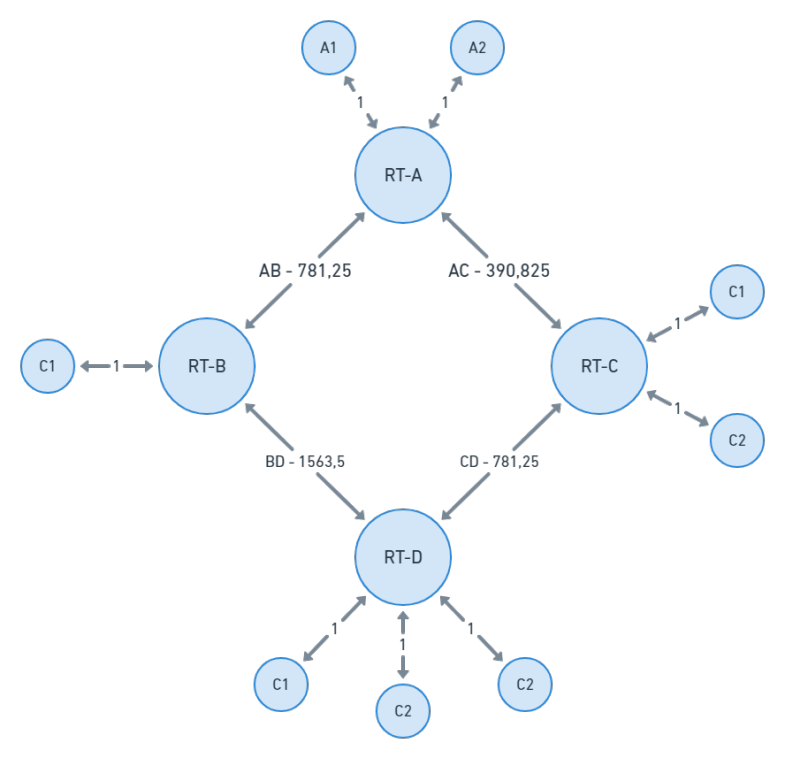
\includegraphics[scale=0.30]{./djikstra_manual.png}
			\end{center}
			\caption{Network topology in regards to travel cost}
		\end{figure}

		\subsubsection{Each group member will now select one of the four routers, and from this router calculate the shortest path to all the sub-networks using Dijkstra's algorithm. What are the costs to reach the different networks?}


		\begin{figure}[H]
			\begin{center}
			\begin{tabular}{|c|c|c|}
				\hline
Route & Path & Cost \\ 
				\hline
A → A1 & A → A1 & 1 \\ 
				\hline
A → A2 & A → A2 & 1 \\ 
				\hline
A → AC & A → AC & 0 \\ 
				\hline
A → C & A → AC → C & 390,625 \\ 
				\hline
A → C1 & A → AC → C → C1 & 391,625 \\ 
				\hline
A → C2 & A → AC → C → C2 & 391,625 \\ 
				\hline
A → CD & A → AC → C → CD & 390,625 \\ 
				\hline
A → D & A → AC → C → CD → D & 1171,875 \\ 
				\hline
A → D1 & A → AC → C → CD → D → D1 & 1172,875 \\ 
				\hline
A → D2 & A → AC → C → CD → D → D2 & 1172,875 \\ 
				\hline
A → D3 & A → AC → C → CD → D → D3 & 1172,875 \\ 
				\hline
A → BD & A → AB → B → BD & 781,25 \\ 
				\hline
A → B & A → AB → B & 781,25 \\ 
				\hline
A → B1 & A → AB → B → B1 & 782,25 \\ 
				\hline
A → AB & A → AB & 0 \\ 
				\hline
				\end{tabular}
				\caption{RT-A}
			\end{center}
		\end{figure}

		\begin{figure}[H]
			\begin{center}
			\begin{tabular}{|c|c|c|}

				\hline
Route & Path & Cost \\
\hline
B → B1 & B → B1 & 1 \\
\hline
B → AB & B → AB & 0 \\
\hline
B → A & B → AB → A & 781,25 \\
\hline
B → A1 & B → AB → A → A1 & 782,25 \\
\hline
B → A2 & B → AB → A → A2 & 782,25 \\
\hline
B → AC & B → AB → A → AC & 781,25 \\
\hline
B → C & B → AB → A → AC → C & 1171,875 \\
\hline
B → C1 & B → AB → A → AC → C → C1 & 1172,875 \\
\hline
B → C2 & B → AB → A → AC → C → C2 & 1172,875 \\
\hline
B → CD & B → AB → A → AC → C → CD & 1171,875 \\
\hline
B → D & B → BD → D & 1582,5 \\
\hline
B → D1 & B → BD → D → D1 & 1583,5 \\
\hline
B → D2 & B → BD → D → D2 & 1583,5 \\
\hline
B → D3 & B → BD → D → D3 & 1583,5 \\
\hline
B → BD & B → BD & 0 \\
\hline

			\end{tabular}
			\caption{RT-B}
			\end{center}
		\end{figure}

		\begin{figure}[H]
			\begin{center}
			\begin{tabular}{|c|c|c|}


				\hline
Route & Path & Cost \\
\hline
C → A1 & C → AC → A1 & 391,625 \\
\hline
C → A2 & C → AC → A2 & 391,625 \\
\hline
C → AC & C → AC & 0 \\
\hline
C → C1 & C → C1 & 1 \\
\hline
C → C2 & C → C2 & 1 \\
\hline
C → CD & C → CD & 0 \\
\hline
C → D & C → CD → D & 781,25 \\
\hline
C → D1 & C → CD → D → D1 & 782,25 \\
\hline
C → D2 & C → CD → D → D2 & 782,25 \\
\hline
C → D3 & C → CD → D → D3 & 782,25 \\
\hline
C → BD & C → CD → D → BD & 781,25 \\
\hline
C → B & C → AC → A → AB → B & 1171,875 \\
\hline
C → B1 & C → AC → A → AB → B → B1 & 1172,875 \\
\hline
C → AB & C → AC → A → AB → B → B2 & 1172,875 \\
\hline
C → A & C → AC → A & 390,625 \\
\hline
			\end{tabular}
			\caption{RT-C}
			\end{center}
		\end{figure}

		\begin{figure}[H]
			\begin{center}
				\begin{tabular}{|c|c|c|}
					\hline
	Route & Path & Cost \\
	\hline
	D → A1 & D → CD → C → AC → A → A1 & 1172,875 \\
	\hline
	D → A2 & D → CD → C → AC → A → A2 & 1172,875 \\
	\hline
	D → AC & D → CD → C → AC & 781,25 \\
	\hline
	D → C & D-CD → C & 781,25 \\
	\hline
	D → C1 & D → CD → C → C1 & 782,25 \\
	\hline
	D → C2 & D → CD → C → C2 & 782,25 \\
	\hline
	D → CD & D → CD & 0 \\
	\hline
	D → D1 & D → D1 & 1 \\
	\hline
	D → D2 & D → D2 & 1 \\
	\hline
	D → D3 & D → D3 & 1 \\
	\hline
	D → BD & D → BD & 0 \\
	\hline
	D → B & D → DB → B & 1562,5 \\
	\hline
	D → B1 & D → DB → B → B1 & 1563,5 \\
	\hline
	D → AB & D → CD → C → AC → A → AB & 1171,875 \\
	\hline
	D → A & D → CD → C → AC → A & 1171,875 \\
	\hline
				\end{tabular}
				\caption{RT-D}
			\end{center}
		\end{figure}

		\subsubsection{Issue the command show ip route and look at the metric OSPF use for all the networks in the routing table. Are the metrics the same as the metrics you calculated in question 2?}

		The RT-A and RT-B seems to have the same values as the calculated one’s we got using dijkstra's algorithm. RT-C and RT-D on the other hand seem to have some problems in terms  of that the cost to get to every path is 0. We may have misconfigured the OSPF in some way, but we were able to ping and communicate with all the subnetworks.

		\subsubsection{Issue the ping command from RT-D to the loopback on RT-A. Which path does the ICMP-packet take to reach RT-A loopback?}

		\begin{verbatim}
			RT-D#ping 200.169.248.12
Type escape sequence to abort.
Sending 5, 100-byte ICMP Echos to 200.169.248.12, timeout is 2 seconds:
!!!!!
Success rate is 100 percent (5/5), round-trip min/avg/max = 20/20/24 ms
		\end{verbatim}

		By comparing this RTT to the previous measurements, we can deduce that the package travels through RT-C.

		\subsubsection{Modify the OSPF-metric so that it prefers to send packages though RT-B instead of RT-C when sending packages from RT-D to RT-A. Show how you achieved this.}

		There are two ways to accomplish this. One could either configure RT-B to have a lesser internal distance than compared to RT-C, explicitly suggesting the system to prefer the RT-B path over the RT-C path. One could also change the bandwidth for the interfaces at RT-B or RT-C, which would implcitly cause the system to prefer the RT-B path over the RT-C path. We tried restarting the interfaces after reconfiguring them, but we sadly did not manage to get either of these two configurations to work out in reality, and we do not know why.

		\subsubsection{Which group member was doing the configuration for this part?}

		As in the previous sections, we did all the configuration on one computer and discussed what commands to use for the configuration but this time Adam Temmel was the one pushing the buttons.

\end{document}

